\section*{Глава 1. Основные сведения и постановка задачи}
\addcontentsline{toc}{section}{Глава 1. Основные сведения и постановка задачи}
\setcounter{section}{1}

\subsection{Общие факты}

Глубокое обучение - это быстрорастущая часть машинного обучения, которая является подвидом искусственного интеллекта (ИИ), ставшая очень популярной в последние годы. Именно с помощью данного подхода, было разработано большое количество различных алгоритмов, связанных с компьютерным зрением, распознаванием речи, прогнозированием данных и другими сложными задачами [1].

Под глубокой сетью, в данном случае, подразумевается число слоев, через которые преобразуются данные. Таким образом, чем больше слоев в сети, тем глубже считается нейрокомпьютерная сеть. 

Глубокие нейронные сети стали хорошим решением, благодаря своим показателям в области признаков визуальной информации. В отличие от более простых конструкций, когда мы задаем признаки в ручную, многослойная архитектура может более эффективно описать исходный набор данных.

Одним из типов глубоких нейронных сетей являются сети глубокого доверия (ГСД). Данная модель нейронных сетей состоит из нескольких скрытых слоев, в каждом из которых нейроны не связаны между собой, но связаны с нейронами соседнего слоя. Таким образом, выполняя обучение на наборе примеров спонтанным образом, ГСД может обучаться и вероятностно отстраивать свои входы. Одна из таких моделей будет рассмотрена на задаче отслеживания траектории объекта.

Отслеживание объекта относится к автоматической оценке траектории при его перемещении на видео. Также отметим, что задача может требовать отслеживания нескольких объектов, но она все равно сводится к обработке каждого объекта в отдельности. Видео обычно представляется набором изображений. Помимо этого, может иметься набор значений к каждому изображению, которые задают действительное положение объекта. Второе используется для оценки работы данного алгоритма, чтобы оценить его точность и правильность в различных ситуациях.

После того, как отслеживаемый объект идентифицируется вручную или автоматически в первом видео-кадре, цель данного алгоритма состоит в том, чтобы автоматически вычислять траекторию движения объекта в последующих кадрах, то есть определять центр отслеживаемого объекта.

Большинство существующих моделей используют либо генеративный, либо дискриминационный подход. Генеративные модели, как и другие модели в машинном обучении с таким же понятием, предполагают, что отслеживаемый объект может быть описан некоторым генеративным процессом, и, следовательно, отслеживание заключается в поиске более вероятного кандидата среди, возможно, бесконечного множества. Так, например, генеративными моделями являются модели, описанные в статье [2].

С другой стороны, дискриминационный метод рассматривает данную задачу как проблему двоичной классификации, которая учится явно отличать отслеживаемый объект от его фона. К этой категории моделей относится online-трекер AdaBoost (OAB) [3].

В то время как генеративные методы обычно дают более точные результаты в менее сложных средах из-за более богатых представлений изображения, дискриминационные методы более устойчивы к сильным окклюзиям и вариациям, поскольку они явно учитывают фон [4].

В дальнейшем, в работе будут рассматриваться генеративные подходы к решению задачи слежения за объектами с помощью сетей глубокого доверия.

\subsection{Анализ существующих алгоритмов}

Рассмотрев уже существующие трекеры, например, описанные  в статьях [5] и [6], которые реализуют поставленную общую задачу отслеживания, нетрудно отметить их самый большой минус -- большие затраты на вычисление; они являются очень трудоемкими, объемными, что крайне не подходит, например, для онлайн-решения задачи.

Данное суждение приводит к поиску и аналитике альтернативных существующих алгоритмов. В ходе данной работы были рассмотрены следующие алгоритмы:

\begin{itemize}[leftmargin=0em, itemindent=2.5 em,itemsep=1.5 pt,parsep=1.5 pt]

\item[--] алгоритм глубокого обучения (DLT) и его программная реализация, описанная в статье [7]. Данный подход состоит из обучения с учителем глубокой сети, а затем онлайн-обучении во время непосредственного применения на конкретной последовательности. Именно данный алгоритм разбирается подробнее и на нем исследуется влияние квантования весов, по причине его хороших результатов в отслеживании объектов. Рассмотрим подробнее устройство данного алгоритма в следующих параграфах;

\item[--] алгоритм регионального глубокого обучения (RDLT), описанный в статье [8]. Данный алгоритм является своеобразным усложнением предыдущего. Взяв за основу схожие методы DLT, авторы усложнили его путем разделения целостной рамки, которая следит за объектом, на k частей;

\item[--] эталонный тест производительности [3], для сравнения существующих моделей между собой. В данной программе содержится 29 известных алгоритмов слежения, реализованных на основе оригинальных статей создателей методов, с одинаковыми  входными данными для чистоты эксперимента. В данную программу можно добавить модель, для сравнения, в частности в нее включена модель DLT.

\end{itemize}

Данная аналитика приводит нас к дальнейшему более подробному анализу работы алгоритма DLT, в частности его основных подходов и методов.

\subsection{Математическая модель DLT}
\subsubsection{Подход фильтр-частиц} 

Фильтр-частицы - частый генеративный подход к задаче отслеживания траектории движения. С точки зрения статистики, это последовательный метод выбора важности по методу Монте-Карло для оценки переменных скрытого состояния динамической системы на основе последовательности предыдущих наблюдений. Так, например, данный подход используется в реализации моделей DLT  и RDLT. Далее опишем основную идею данного метода.

Пусть $s^{t}$ и $y^{t}$ обозначают скрытое состояние и переменное наблюдение в момент времени $t$ (\ref{eq1}). Математически, отслеживание объекта, как мы уже говорили ранее, -- это задача о нахождении наиболее вероятного состояния для каждого временного шага t на основе наблюдений до предыдущего временного шага:

\begin{equation}\label{eq1}
    s^{t} = argmax(p(s^t|y^{1:t-1}))
\end{equation}

То есть, это такой аргумент функции вероятности в момент $t$ при условии предыдущих наблюдений, что функция на нем перенимает максимальное значение. После данной обработки, распределение переменной состояния обновляется в соответствии с правилом Байеса (\ref{baes}):

\begin{equation}\label{baes}
    p(s^t|y^{1:t}) = \dfrac{p(y^t|s^t)p(s^t|y^{1:t-1})}{p(y^t|y^{1:t-1})} 
\end{equation}

Исходя из формулы (\ref{baes}), аппроксимируем выражение слева с помощью набора $\{s^{(i)}_t\}^{n}_{i=1}$ дискретной конечной выборки, называемой частицами, с соответствующими весами (\ref{eq3}).

\begin{equation} \label{eq3}
    w^{(i)}_{t}=w^{(i)}_{t-1}\dfrac{p(y_t|s^{(i)}_t)p(s^{(i)}_t|s^{(i)}_{t-1})}{q(s_t|s_{1:t-1},y_{1:t})}
\end{equation}

В случае, если сумма весов меньше порогового значения, применяется повторная выборка, чтобы извлечь $n$ частиц из текущего набора частиц пропорционально их весу, а затем сбросить их веса до $\dfrac{1}{n}$. Если сумма весов превышает пороговое значение, применяется линейная нормализация, чтобы гарантировать, что сумма весовых коэффициентов равна 1. 

Для отслеживания объекта, переменная состояния $s_i$ обычно представляет собой шесть параметров аффинного преобразования: сдвиг, масштаб, соотношение сторон и поворот.

В частности, каждое измерение $q(s_t|s_{t-1})$ независимо моделируется нормальным распределением. Для каждого кадра результатом отслеживания является просто частица с наибольшим весом.

Структура фильтр-частиц является распространенным подходом в визуальном отслеживании. Она аппроксимирует распределение апостериорных состояний по множеству частиц, а не только по одной точке. Для визуального отслеживания это свойство облегчает модели восстановление после неверных результатов отслеживания.

\subsubsection{Предобработка данных}

Модель DLT представляет собой алгоритм, с помощью которого можно обработать в режиме реального времени последовательность изображений, определив на каждом из них центр отслеживаемого объекта. При поступлении изображений в модель, последовательность должна подать на вход программы вектор с координатами объекта на первом кадре (в пикселях), ширину и высоту объекта, и угол, на который повернут начальный объект. Также необходим аналогичный вектор с предполагаемым начальным сдвигом.

Далее производится нормализация данных, а именно ширина и высота отслеживаемого видео кадра приводится к разрешению 320 на 240, это нужно иметь ввиду при подаче последовательности в данный алгоритм. В случае если входная последовательность не находится в черно-белом формате она в него переводится, для уменьшения количества входных данных. Таким образом, мы можем напрямую использовать цветные изображения, при необходимости.

Также, для инициализации самой нейросети на нормализованных данных, необходимо загрузить обученные весовые коэффициенты сети. Данные матрицы были получены с помощью набора данных Tiny Images [9] -- вспомогательные данные для автономного обучения. Набор данных охватывает многие объекты и сцены, найденные в реальном мире. Из почти 80 миллионов крошечных изображений, каждое из которых имеет разрешение 32 × 32, случайным образом отобрали миллион изображений на которых было произведено обучение. На данном этапе в автономном режиме обучение выполняется путем шумоподовляющего автоэнкодера с накоплением (SDAE) для изучения общих характеристик в нем. Данная конструкция как раз относится к сетям глубокого доверия. Для более подробного описание этапа автономного обучения сети необходимо обратиться к статье [7].

\subsubsection{Онлайн обучение нейронной сети}

После произведенной пред-обработки данных, описанной выше, происходит этап онлайн обучения. Отметим сразу, что при выполнении данного, время работы сети заметно увеличивается, из-за дополнительного прохода по ней.

 \begin{figure}[h!]\label{arh}
    \centering
    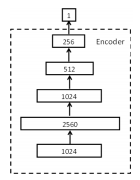
\includegraphics[width = 6 cm]{tests/img/online.PNG}
    \caption*{Рисунок 1.1 - Архитектура online-обучения DLT}
\end{figure}

Для первичного кадра последовательности происходит формирование 10 позитивных и 100 негативных примеров, на которых будет производиться онлайн обучение нейронной сети. Некоторые негативные примеры собраны из фона на небольшом расстоянии от объекта. Далее происходит инициализация сети, подгружается обученная матрица весовых коэффициентов. На основе полученных данных строится сигмоидальный классификационный слой, который добавляется в архитектуру SDAE (Рисунок 1.1), полученную в результате автономного обучения.

Базовым строительным блоком SDAE является однослойная нейрокомпьютерная сеть, которая называется автоинкодером с шумоподавлением (DAE). Она является более поздним вариантом обычного автоэнкодера и учится восстанавливать образец данных из его поврежденной версии. 

После этого, для вычисления коррекции весовых коэффициентов матрицы, выполняется алгоритм обратного распространения ошибки, после чего завершается этап инициализации нейронной сети.

Кроме того, стоит добавить, что когда считывается новый видео-кадр, сначала вычисляются фильтр-частицы в соответствии с подходом, описанным выше, а затем достоверность каждой частицы определяется путем простого прямого прохода через сеть. 

\subsection{Квантование весов}

Известно, что реализация нейронной сети задействует много памяти для хранения, как минимум, матрицы весов для каждого слоя нейронов. Так как рассматривается глубокое обучение -- множество матриц перехода, из-за чего хранение является дорогостоящей опцией.

Данную проблему можно решить с помощью использования вместо ячейки памяти - мемристора. Задача квантования весов, описанная в статье [10], которая является ключевой в данной работе, использует их для аппаратной реализации весов нейронной сети. Многоуровневые мемристоры реализуют множество дискретных уровней проводимости (иначе говоря, значение мемристора может принимать L значений числа уровней квантования). Они основаны на механизме переключения, а также, достаточно широко распространены, в отличие от аналоговых мемристоров с непрерывной проводимостью. В настоящей работе, необходимо отметить, что многоуровневые мемристоры устойчивы к различным статистическим отклонениям по сравнению с аналоговыми. 

% Перевод данных об алгоритмах
	\renewcommand{\listalgorithmname}{Список алгоритмов}
	\floatname{algorithm}{Алгоритм}
	
	% Перевод команд псевдокода
	\algrenewcommand\algorithmicwhile{\textbf{До тех пока}}
	\algrenewcommand\algorithmicdo{\textbf{выполнять}}
	\algrenewcommand\algorithmicrepeat{\textbf{Повторять}}
	\algrenewcommand\algorithmicuntil{\textbf{Пока выполняется}}
	\algrenewcommand\algorithmicend{\textbf{Конец}}
	\algrenewcommand\algorithmicif{\textbf{Если}}
	\algrenewcommand\algorithmicelse{\textbf{иначе}}
	\algrenewcommand\algorithmicthen{\textbf{тогда}}
	\algrenewcommand\algorithmicfor{\textbf{Цикл}}
	\algrenewcommand\algorithmicforall{\textbf{Выполнить для всех}}
	\algrenewcommand\algorithmicfunction{\textbf{Функция}}
	\algrenewcommand\algorithmicprocedure{\textbf{Процедура}}
	\algrenewcommand\algorithmicloop{\textbf{Зациклить}}
	\algrenewcommand\algorithmicrequire{\textbf{Условия:}}
	\algrenewcommand\algorithmicensure{\textbf{Обеспечивающие условия:}}
	\algrenewcommand\algorithmicreturn{\textbf{Возвратить}}
	\algrenewtext{EndWhile}{\textbf{Конец цикла}}
	\algrenewtext{EndLoop}{\textbf{Конец зацикливания}}
	\algrenewtext{EndFor}{\textbf{Конец цикла}}
	\algrenewtext{EndFunction}{\textbf{Конец функции}}
	\algrenewtext{EndProcedure}{\textbf{Конец процедуры}}
	\algrenewtext{EndIf}{\textbf{Конец условия}}
	\algrenewtext{EndFor}{\textbf{Конец цикла}}
	\algrenewtext{BeginAlgorithm}{\textbf{Начало алгоритма}}
	\algrenewtext{EndAlgorithm}{\textbf{Конец алгоритма}}
	\algrenewtext{BeginBlock}{\textbf{Начало блока. }}
	\algrenewtext{EndBlock}{\textbf{Конец блока}}
	\algrenewtext{ElsIf}{\textbf{иначе если }}
	
	\begin{algorithm}[h!]
		\begin{algorithmic}[1]
			\State Находим максимальный по модулю элемент матрицы весов $W_{max}$
			\State $\Delta = \frac{W_{max}}{L-1}$
			\For{ по всем элементам $W_{ij}$}
			\For{\textbf{от} $k=0$ \textbf{до} L}
			\If{$(k-1) \Delta < |W_{ij}| < k \Delta$}
			\State $W{ij} = (k-1) \Delta sign(W_{ij})$
			\EndIf
			\EndFor
			\EndFor
		\end{algorithmic}
	\caption*{Алгоритм 1.1 -- Алгоритм квантования весовых коэффициентов}
	\end{algorithm}
	
Для реализации задачи квантования необходимо после пред-обучения нейронной сети и заполнения матрицы весов, при запуске частного случая, а именно после загрузки весов обученной сети, провести квантование данной матрицы. Алгоритм квантования весов (Алгоритм 1.1) заключается в замене весовых коэффициентов матрицы на аппроксимированные значения в зависимости от уровней квантования. 

Для квантования весов необходимо также определиться с числом уровней квантования. Поиск данного числа предлагается искать опытным путем через сравнение с исходными значениями алгоритма слежения. 
